\chapter{介绍}
	在数据中查找模式的问题是一个基础性问题,并且有很长而成功的历史。例如,Tycho Brahe在16世纪广泛的天文观察是的开普勒发现了天体运动规律,这又提供了经典力学发展的跳板。同样的,原子光谱规律的发现也对量子物理的发展和验证起到了关键的作用。模式识别领域关注于使用计算机算法来自动地发现数据中的规律,并且使用这些规律进行如对不同类别进行分类的一些活动。
	
	思考手写数字的识别例子,如图1.1。每个数字对应$28 \times 28$个像素,可以使用包含784个实数的向量$\mathbf{x}$来表示。目标是去构建一个机器,向量$\mathbf{x}$作为输入,产生数字$0,\dots, 9$作为输出。可以使用手工规则或者启发式来根据笔画形状来区分数字,但是这种方法在实践中会导致增加例外的规则,并且不约而同地给出糟糕的结果。
	
\begin{figure}
	\centering
	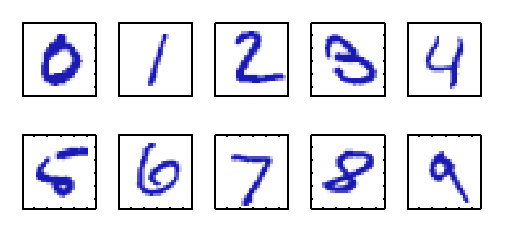
\includegraphics[width=8cm]{Figure1-1.eps}
	\caption{Examples of hand-written digits taken from US zip codes} 
	\label{fig:endb-flow} 
\end{figure}

	更优的结果是采用机器学习方法,这种方法中有一个很大的数字集合N $\{ \mathbf{x_1},$ $ \dots, \mathbf{x_N} \}$ 称为训练集,用来调整得到可适应模型的参数。在训练数据集中的数字分类已经提前给出,通常通过单独手工贴标签来检查他们。我们可以使用目标向量$\mathbf{t}$来表达一个数字的分类,表示对应数字的定义。对于用向量来表示的类别技术会在后面来进行讨论。注意到这里对于每一个数字图像$\mathbf{x}$,使用一个目标向量来表示。
	
	机器学习算法运行的结果可以表示为一个函数$\mathbf{y(x)}$,函数使用一个新的数字图像$\mathbf{x}$作为属兔,产生一个输出向量$\mathbf{y}$,其和目标向量的编码相同。函数$\mathbf{y(x)}$的精确格式在基于训练数据训练阶段时候确定,也被称作学习阶段。当模型确定后,就可以用来确定一个新的的数字图像,包括一个测试数据集。新样本的分类正确性不同于用来训练数据样本的能力称作\textbf{一般化}(generalization)。在实践应用中,输入的各种各样向量使得训练数据可以包含所有可能输入向量的极小部分,并且这也是模式识别的中心目标。
	
	对于大多数的实践应用,原始输入变量都预处理为新空间的变量,是为了希望可以可以很容易地解决模式识别问题。例如,在数字识别问题中,数字的图像通常被转化或者规范化,从而使得每个数字可以在一个固定大小的框中。这可以减少数字类中的变量,因为数字的位置和规模都相同了。这更容易使用子序列模式识别算法在不同类中区别进行区别。这种预处理阶段有时候称为\textbf{特征提取}(f\textit{eature extraction})。注意到测试数据必须和训练数据一样使用同样的步骤进行预处理。
	
	预处理也会用来提高计算性能。例如,如果目标是在高速视频流的实时人脸检测,计算机必须每秒处理大量的像素,并且直接展示这给一个复杂的模式识别算法或许计算不可行的。代替地,发现有用特征的目标是能计算更快,并且还保留有用的区别信息来使得可以区别人脸和非人脸。这些特征作为模式识别算法的特征。例如,在矩形子区域上的图像强度均值可以非常有效地进行评估,并且一个特征集可以在快速人脸检测上非常有效。因为这些特征的数量比像素点更少,这种预处理表达了降维的一种形式。必须注意到在预处理过程中,因为信息的丢弃,如果这个信息对于处理问题是重要的,那就可以会遭受系统整体精度的痛苦。
	
	训练数据包含的样本是输入向量对于目标向量的应用是\textbf{监督学习}(\textit{supervised learning})问题。例如数字识别样本,其中的目标是将每个输入向量赋值为一个有限的离散数字,称为\textbf{分类问题}(\textit{classification})。如果期望的输出包含一个或多个连续的变量,这种任务称为\textbf{回归}(\textit{regression})。分类问题的一个例子是预测化工生产过程的产率,其中输入包裹关注的反应物,温度和压强。
	
	在其他的模式识别问题中,训练数据包含一个输入向量集$\mathbf{x}$,没有对应任何的目标值。在这种非监督学习(unsupervised learning)问题可能会在数据中发现一组相同样本,称为\textbf{聚类}(clustering),或者在一个输入空间中确定一个数据的分布,称为\textbf{密度估计}(\textit{density estimation}),或者将高维数据空间投影到两三维,目的是\textbf{可视化}(\textit{visualization})。
	
	最后,\textbf{加强学习}(\textit{reinforcement learning}, Sutton and Barto, 1998)的技术关注的问题是在给定的语境下采取合适的方法去最大化奖励。对于监督学习,学习算法不会输出一个最优的样本,但必须通过实验和错误来发现他们。通常情况下存在一系列的状态和动作,其中学习算法与它的环境交互。在很多例子中,现有的动作不仅仅影响现在的奖励,并且也会对所有的子序列时间步骤产生影响。例如,通过加强学习的技术,神经网络可以学习到下西洋双陆棋达到一个很高的标准(Tesauro,1994)。在这里,网络必须学会将棋盘的一个随机位置作为输入,接着产生一个强的的移动作为输出。这通过将网络与其自己的一个拷贝来对抗来完成,或许会进行百万次。一个主要的挑战是西洋双陆棋会包含很多种移动,只有在游戏结束的时候,在取得胜利的情况下,奖励才得以实现。奖励必须适当地对所有的移动产生贡献,即使一些移动会有好的情况但其他的会差些。这是一种\textbf{信贷分配}(\textit{credit assignment})问题。加强学习的一个通常的特征是\textbf{探索}(\textit{exploration})和\textbf{开发}(\textit{exploitation})之间的权衡,其中探索是系统尝试新的方法来观察他们将会有怎样的效果,而开发系统会使用已知的动作来产生高的奖励。太关注探索或者开发都将会差生较差的结果。加强学习任然是机器学习研究中一个活跃的课题。然而,详细的讨论会超出本书的范围。
	
	尽管每个问题都需要自己的工具和技术,但是很多关键的想法都支撑着所有的这些问题。这章主要的目标是用相关的非形式化方法去介绍介个最重要的的概念和用简单的例子描述他们。在书的后面,我们将会看到这些想法在再出现在更加复杂的模型中,这些模型会适用于真实世界的模式识别中。这章还会包含三个重要工具的介绍,它们会在整本书中都用到,叫做概率理论,决策理论和信息理论。尽管这些听起来像令人畏惧的话题,但是它们事实上是直接的,并且如果将机器学习技术用到实践应用中,清晰地理解它们是必要的。
	
{ \color{blue} \section{例子:多项式曲线拟合} }
	我们通过引入一个简单的回归问题来开始,我们将会用它作为一个运行的例子来贯穿整章来激励一些关键概念。假设我们观察一个真实值输入变量$x$,我们希望使用这个观察值去预测真实值目标变量$t$的值。对于目前的目的,使用合成的方法产生人造样本是具有启发性的,因为当我们进行学习模型比较时候,我们能知道生成数据的精确过程。样本的数据是由在目标值中包含随机噪声的的函数$sin(2 \pi x)$产生的,具体描述见附录A.

	现在假设我们有一个训练集$\mathbf{x} \equiv (x_1, \dots x_N)^T $,包含N个x的观察值,对应的t的观察值表示为$\mathbf{t} \equiv (t_1, \dots t_N)^T $。图1.2展示了包含 N = 10 的训练集的点图。图1.2中的输入数据集$\mathbf{x}$是选择$x_n$的值产生的,对于$n = 1, \dots ,N$,取值范围为[0,1],目标数据集$\mathbf{t}$是通过计算函数数$sin(2 \pi x)$得到的对应值,并对每一个点添加一个低水平的服从高斯分布随机噪声(高斯分布会在1.2.4节介绍)可得到$t_n$。通过这种方式产生数据,我们可以得到很多真实数据集的性质,也就是说这些数据存在潜在的规律,我们希望去学习这种规律,但这种独立的观察值受到随机噪声的干扰。这种平噪声可能从本质上体现随机过程,例如放射性衰变,但是通常是因为变量本省是不可观测的。
	
\begin{figure}
	\parbox{.4\textwidth}{\caption{Plot of a training data set of N = 10 points, shown as blue}}
	\parbox{.5\textwidth}{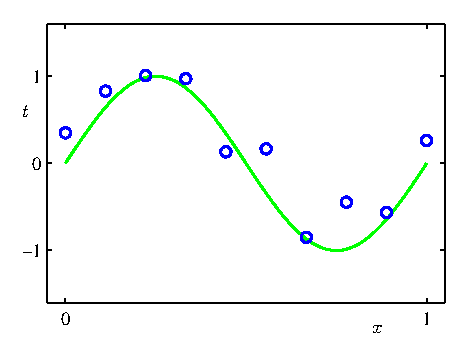
\includegraphics[width=8cm]{Figure1-2.eps}}
\end{figure}

	我们的目标是通过利用训练集,对于一些新的输入变量$\hat{x}$做出预测变量的目标值$\hat{t}$.我们后面可以看到的,这包含隐含地试图找到潜在函数$sin(2 \pi x)$.当我们从有限的数据集中概括时,在本质上是一个棘手的问题。更多的,观察数据集受到噪声的干扰,因此对于一个给定的$\hat{x}$,对应的近似值$\hat{t}$是不确定的。在1.2节中讨论的概率理论提供了一个用精确和定量的方法来表达这种不确定性的框架,在1.5节中讨论的决策理论重现了这种概率的利用,为了根据似然准则做出优化决策。
	
	就目前而言,我们将会非正式地进行和考虑基于曲线拟合的的简单方法,我们使用多项式函数来拟合数据得到形式
	
	\begin{equation}
	y(x,\mathbf{w}) = w_0 + w_1x + w_2x^2 + \dots + w_Mx^M = \sum_{j = 0}^{M}w_jx^j
	\end{equation}
	
	其中M是多项式的阶,$x^j$表示x的j次幂。多项式的系数$w_0, \dots ,w_M$可以使用向量$\mathbf{w}$表示。注意,尽管多项式函数$y(x,\mathbf{w})$是x非线性的函数,但对于w是线性函数。如多项式之类的函数,对于未知参数是线性的,具有重要的性质,称为线性模型,我们将会在3.4节来扩展介绍。
	
	参数的值由对训练数据的多项式拟合确定。这可以表示为通过最小化误差函数(error function),对于任意的值$\mathbf(w)$和训练集数据点,误差函数用来测量函数$y(x,\mathbf{w})$的失配。简单选择被广泛地使用误差函数,通过对每个数据点$x_n$的预测值$y(x,\mathbf{w})$和对应的目标值$t_n$误差平方和,因此我们最小化
	
	\begin{equation}
	E(w) = \frac{1}{2} \sum_{n = 1}^{N}\{ y(x_n,\mathbf{w}) - t_n\}^2
	\end{equation}
	
	其中包含的因子1/2是为了后面计算的方便。我们将会在这个章节的后面讨论使用这个误差函数的原因。现在我们简单地注意到它是一个非负的的等式,当且仅当函数$y(x,\mathbf{w})$精确地通过每一个训练数据点的时候为0。函数平方误差和的几何解析表示为图1.3。
	
	
\begin{figure}
	\parbox{.4\textwidth}{\caption{The error function (1.2) corresponds to (one half of) the sum of the squares of the displacements (shown by the vertical green bars) of each data point from the function $y(x,\mathbf{w})$ } }
	\parbox{.5\textwidth}{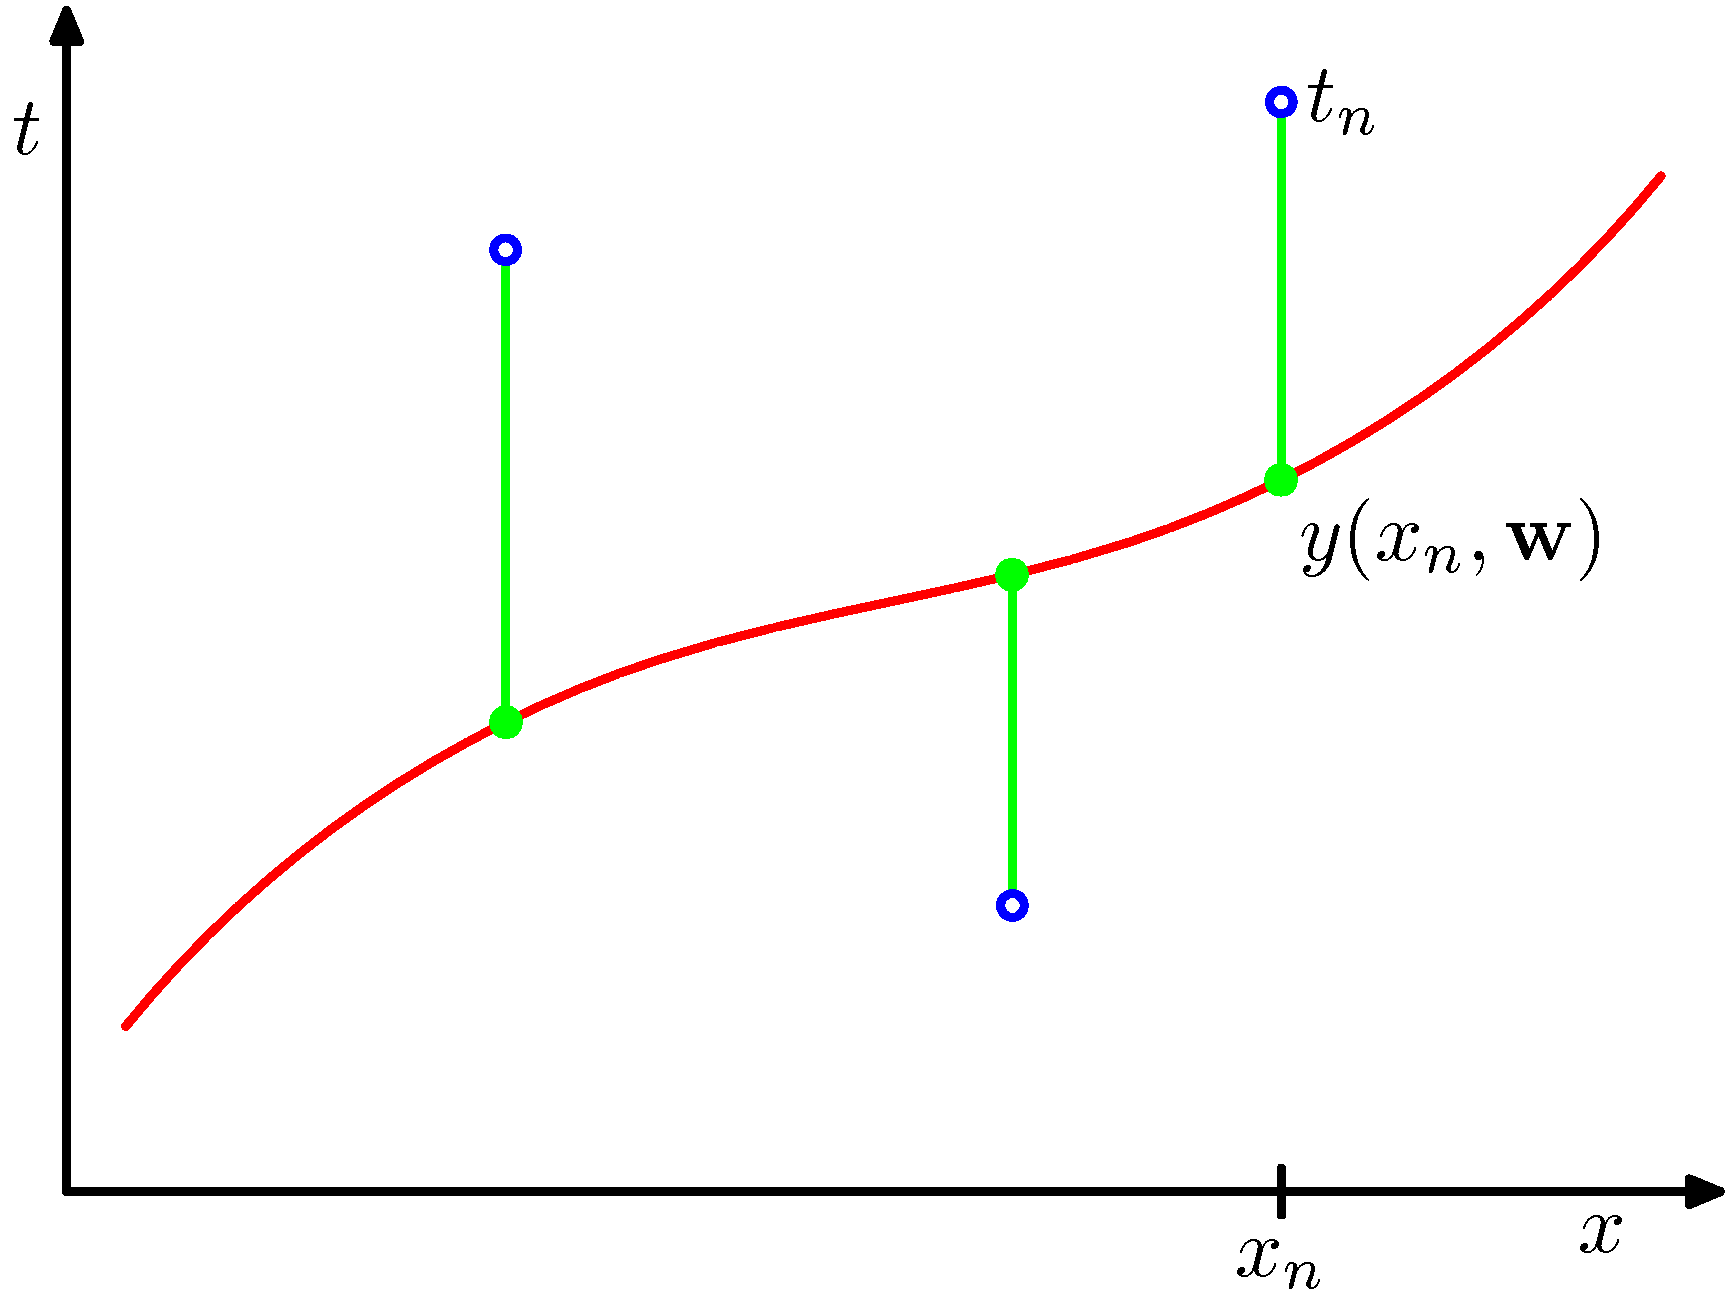
\includegraphics[width=8cm]{Figure1-3.png}}
	\label{fig:endb-flow} 
\end{figure}

	我们可以通过选择$\mathbf{w}$的值来解决曲线拟合问题,其中$E(\mathbf{w})$尽可能小。因为误差函数是参数为$\mathbf{w}$的一个二次函数,它的导数是相对于系数在元素$\mathbf{w}$下是线性的,因此最小化误差函数有唯一的解,可以用紧凑的形式表示为$\mathbf{w}^{\star}$。多项式的结果表示为函数$y(x,\mathbf{w}^{\star})$。
	
	这里存在的问题是如何选择多项式的阶M,我们会看到这会转化为一个重要概念的例子,称为模型对比和模型选择(model comparison or model selection)。在图1.4中,我们展示了对于图1.2中展示的数据集的多项式拟合结果的4个例子,其中多项式的阶数为M = 0,1,3,9。

\begin{figure}[t]
	
	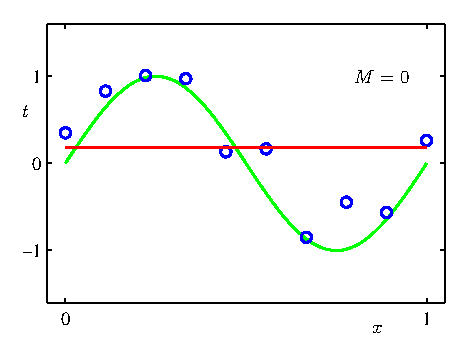
\includegraphics[width=8cm]{Figure1-4a.eps}
	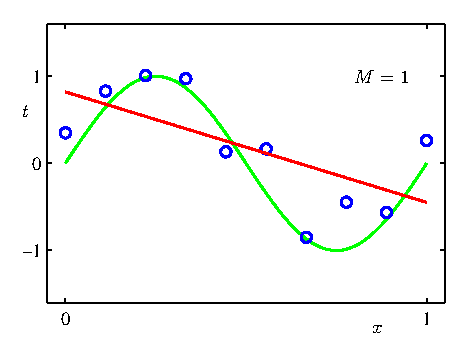
\includegraphics[width=8cm]{Figure1-4b.eps}
	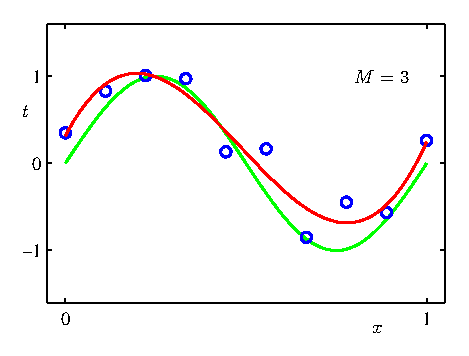
\includegraphics[width=8cm]{Figure1-4c.eps}
	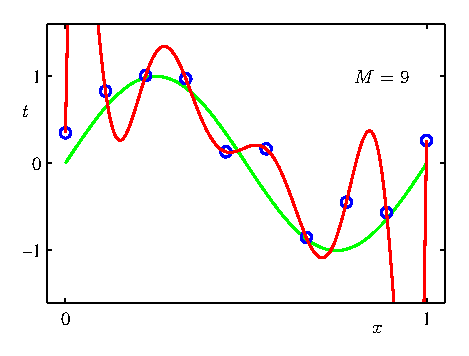
\includegraphics[width=8cm]{Figure1-4d.eps}
	\caption{Plots of polynomials having various orders M, shown as red curves, fitted to the data set shown in
		Figure 1.2. } 
\end{figure}

	我们注意到常量(M = 0)和一次(M = 1)的多项式对于数据得到相当糟糕的拟合,并且对于函数$sin(2 \pi x)$表示也表现很差。如图1.4所示的例子,三次多项式对于函数$sin(2 \pi x)$似乎得到了最好的拟合。当我们采用更高次的多项式(M = 9)时,对于训练数据,我们得到了一个较好的拟合。事实上,多项式精确地通过每个点,并且$E(\mathbf{w}^{\star}) = 0$。反而,拟合曲线较大范围的波动对于函数$sin(2 \pi x)$会得到较差的表示。后面这种行为称为过拟合(over-fitting)。
	
	正如我们前面所描述的,我们的目标是实现对于新数据的精确预测的归纳。我们可以通过考虑单独的测试数据集定量地对这些在M上独立的归纳模型的性能进行观察,其中每个数据集精确地使用和生成训练数据集相同的方法生成的100个数据点,但在目标值中使用新的随机噪声。对于每个选择的M,我们可以对训练数据通过(1.2)式子来评价得到的值$E(\mathbf{w}^{\star})$,并且我们也可以对于测试数据集来评价$E(\mathbf{w}^{\star})$。通常我们使用均方根误差(RMS)来定义更加方便
	
	\begin{equation}
	E_{RMS} = \sqrt{2E(\mathbf{w}^{\star})/N}
	\end{equation}
	
	其中除数M允许我们可以同等地比较不同大小的数据集,并且平方根确保$E_{RMS}$可以和变量t在同一尺度上进行测量。对于不同的M值,训练和测试数据集的REM误差可以在展示在图1.5中。测试数据集是用来测量对于新数据x的观察结果,得到的预测值t的效果如何。我们从图1.5中可以观察到,对于小的M值,会得到相对较大的测试误差。这可以归因于得到的多项式是相当平滑的,并且不能捕获函数$sin(2 \pi x)$的震荡。真如我们所看到的对于图1.4中 M = 3 的例子,M在$3 \leq M \leq 8$范围内时会得到较小的测试误差,并且这也合理地给出了生成函数$sin(2 \pi x)$的表示。

\begin{figure}
	\parbox{.4\textwidth}{\caption{均方根误差的图,定义(1.3),对于不同的M值,用训练集和独立的测试集评估}}
	\parbox{.5\textwidth}{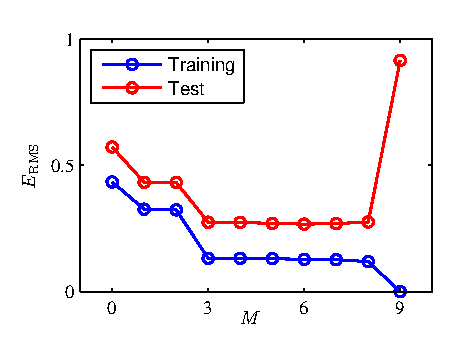
\includegraphics[width=8cm]{Figure1-5.eps}}
	\label{fig:endb-flow} 
\end{figure}

	对于 M = 9,正如我们所预料的,训练集误差为0,因为多项式对应的10个系数包含10个自由度$w_1,\dots,w_9$,所以可以精确地被协调到10个训练数据点。然而,如图1.4所示,测试集误差变得非常大时,对应的函数$y(x, w^{\star})$波动很大。
	
	这似乎是矛盾的,因为一个给定阶数的多项式包含所有低阶的的例子。M = 9 的多项式因此能和 M = 3 的多项式产生一样好的结果。此外,我们或许可以假设对于新数据的最好预测可能是函数来自于函数$sin(2 \pi x)$,其中的数据是由函数生成的(我们后面可以看到这确实是这样的)。我们知道函数$sin(2 \pi x)$的一个幂级数展开包含所有的阶,因此我们期望当我们增加M时,性能会单调地提升。
	
	我们可以通过检验从各种阶数的多项式得到的系数值来得到一些深入的问题,如表1.1所示,我们可以看到,当M增加时,系数的增幅会变得更大。尤其对于M = 9 的多项式,系数完美地在很大的正数和负数之间变换,从而使得多项式函数可以精确地匹配每个数据。但在数据之间,如图1.4中所看到的,函数出现很大的波动。直观地,有很大值M的多项式越平滑,目标值得到的随机噪声越大。
	
	%table1.1
	\begin{table}[b]
		\parbox{.3\textwidth}{\caption{不同阶数的多项式的系数$w^{\star})$,观察当多项式阶数增加时,系数是如何增加的}}
		\parbox{.5\textwidth}{
		\begin{tabular}{r|rrrr}
			& M = 0 & M = 1 & M = 6 & M = 9\\
			\hline
			$w_0^{\star}$ & 0.19 & 0.82 & 0.31 & 0.35 \\
			$w_1^{\star}$ &      & -1.27 & 7.99 & 232.37 \\
			$w_2^{\star}$ &      &       & -25.43 & -5321.83 \\
			$w_3^{\star}$ &  	 & 		 & 17.37 & 48568.31 \\
			$w_4^{\star}$ & 	 & 		 &  	 & -231639.30 \\
			$w_5^{\star}$ & 	 &  	 & 		& 640042.26 \\
			$w_6^{\star}$ & 	 &  	 &  	& -1061800.52 \\
			$w_7^{\star}$ &  	 &  	 &  	& 1042400.18 \\
			$w_8^{\star}$ &  	 &  	 & 		& -557682.99 \\
			$w_9^{\star}$ &  	 & 		 &		&  125201.43
			
		\end{tabular}
	}
	\end{table}
	
	当数据集大小变动时,检验一个给定模型的的行为也是一件有趣的事情,如图1.6所示。我们可以看到,对于一个给定的模型复杂度,当数据集的大小增加时,过拟合问题会变得更小。换句话说,数据集越大时,我们需要的模型就越复杂去拟合数据。一个粗略的启发是,数据点的数量不应该少于模型参数个数的几倍(可能5或者10)。然而,我们可以在第3章中看到,参数的个数并不是衡量模型复杂程度的最合适标准。
	
	\begin{figure}
		
		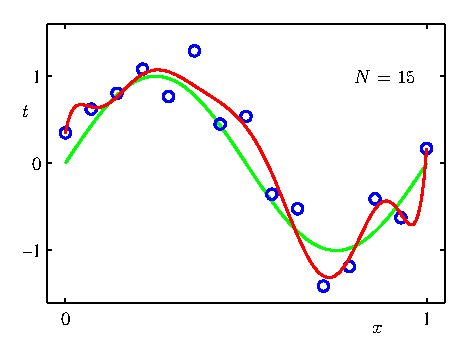
\includegraphics[width=8cm]{Figure1-6a.eps}
		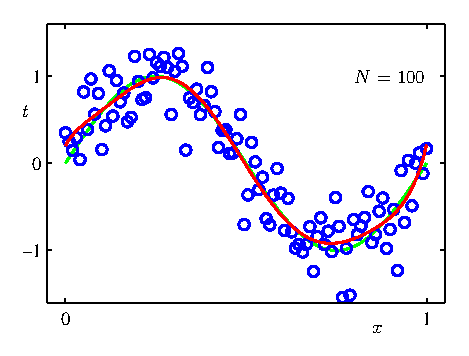
\includegraphics[width=8cm]{Figure1-6b.eps}

		\caption{使用 M =9 的多项式,对于 N = 15(左图) 和 N =100(右图) 的点个数得到的结果,我们可以看到当数据集越大时,过拟合问题越小} 
		\label{fig:endb-flow} 
	\end{figure}
	
	这里也有一些令人很不满意的事,就是必须要根据训练数据集的大小来限制模型参数的个数。这似乎很有道理,根据需要解决的问题的复杂度大小来选择模型的复杂程度。我们可以看到用最小二乘法来找模型参数展现了最大似然估计的一个特殊例子(在1.2.5节中讨论),并且过拟合问题可以理解为最大似然估计的一个通用属性。通过使用贝叶斯方法,过拟合问题可以避免。我们可以发现在模型中利用贝叶斯的方法可以使得参数的个数超过数据点个数。在贝叶斯模型中,真实的参数个数会根据数据集的大小自动调整。
	
	目前,继续用现在的方法和考虑在实践中如何将其应用到有限数据集中是具有指导性意义的,其中我们希望可以使用相对复杂和灵活的模型。通常用来控制过拟合现象的一种技术是归一化(regularization),其中通过添加一个惩罚项到误差函数(1.2)中,可以避免系数达到较大的值。这个惩罚项形式是所有系数的平方和,修改后的误差函数为
	
	\begin{equation}
	\tilde{E}(w) = \frac{1}{2} \sum_{n = 1}^{N}\{ y(x_n,\mathbf{w}) - t_n\}^2 + \frac{\lambda}{2} \parallel \mathbf{w} \parallel^2
	\end{equation}
	
	其中$\parallel \mathbf{w} \parallel^2 \equiv \mathbf{w}^T\mathbf{w} = w_0^2 + w_1^2 + \dots +w_M^2 $,和平方和误差项相比,系数$\lambda$控制正则项的相关重要性。通常系数$w_0$会在归一化中忽略掉,因为将其纳入选择的范围取决于初始变量的选择(Hastie et al., 2001),或者它可以被包含,但是只是归一化它自己的系数(我们将会在5.5.1节详细地讨论这个话题)。式1.4的误差函数可以再次最小化到更接近的形式。这种技术在统计学中称为\textbf{缩减}(\textit{shrinkage})方法,因为减少了系数的值。尤其在二次方程归一化中称为\textbf{岭回归}(r\textit{idge regression})。在神经网络的环境下,这种方法称为\textbf{权值衰减}(\textit{weight decay})。
	
	图1.7展示了9次多项式的拟合结果,数据和之前的一样,但是使用了(1.4)式给出的归一化的误差函数。我们可以看到,对于$\ln \lambda = -18$,过拟合已经被压制了,我们可以得到一个更加接近函数$sin(2 \pi x)$的表达式。然而,当我们使用较大的$\lambda$值时,我们会得到比较差的拟合,如图1.7所示,对于$\ln \lambda = 0$。拟合的多项式对应的系数在表1.2中给出,表明归一化对减少系数的数量级具有所希望的效果。
	
	\begin{figure}
		
		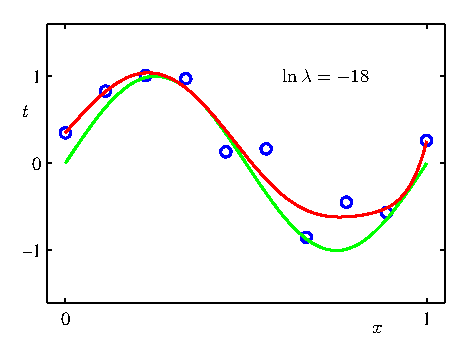
\includegraphics[width=8cm]{Figure1-7a.eps}
		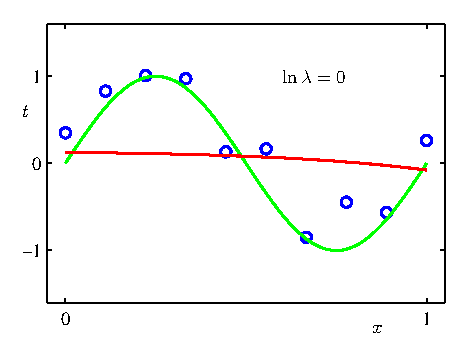
\includegraphics[width=8cm]{Figure1-7b.eps}
		
		\caption{对在图1.2中展示的数据集用M=9的多项式拟合,使用(1.4)的归一化误差函数,两个归一化参数$\lambda$对应$\lambda = -18$ 和$\lambda = 0$} 
		\label{fig:endb-flow} 
	\end{figure}
	
	%table1.2
	\begin{table}[b]
		\parbox{.4\textwidth}{\caption{对于M = 9的多项式,不同的归一化参数$\lambda$值的系数$w^{\star}$。注意当$\ln \lambda = -\inf$时对应的模型没有正则项,即对应图1.4的右下角的图,我们看到,当$\lambda$的值增加时,系数的数量级变得更小}}
		\parbox{.5\textwidth}{
			\begin{tabular}{r|rrr}
				& $\ln \lambda = -\inf$ & $\ln \lambda = -18$ & $\ln \lambda = 0$ \\
				\hline
				$w_0^{\star}$ & 0.35 & 0.35 & 0.13\\
				$w_1^{\star}$ & 232.37 & 4.74 & -0.05 \\
				$w_2^{\star}$ & -5321.83 & -0.77 & -0.06 \\
				$w_3^{\star}$ & 48568.31 & -31.97 & -0.05 \\
				$w_4^{\star}$ & -231639.30 & -3.89 & -0.03 \\
				$w_5^{\star}$ & 640042.26 & 55.28 & -0.02\\
				$w_6^{\star}$ & -1061800.52 & 41.32 & -0.01 \\
				$w_7^{\star}$ & 1042400.18 & -45.95 & -0.00 \\
				$w_8^{\star}$ & -557682.99 & -91.53 & 0.00 \\
				$w_9^{\star}$ & 125201.43 & 72.68 & 0.01
			\end{tabular}
		}
	\end{table}
	
	如图1.8所示,随着$\lambda$的变化,正则项对生成误差的影响可以通过RMS误差的点图看出。我们可以看出$\lambda$控制模型复杂度的效果和确定过拟合的程度。
	
	\begin{figure}[t]
		\parbox{.4\textwidth}{\caption{对于M = 9的多项式,随着$\ln \lambda$的变化的均方根误差图}}
		\parbox{.5\textwidth}{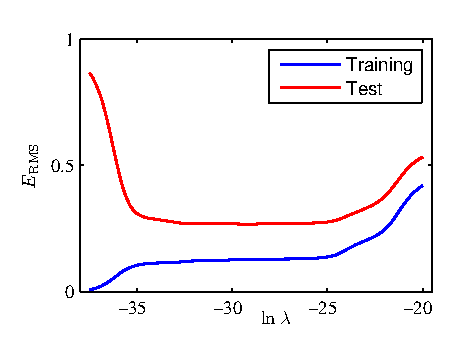
\includegraphics[width=8cm]{Figure1-8.eps}}
	\end{figure}
	
	模型复杂度问题是一个重要的问题,我们会在后面的1.3节详细介绍。这里我们简单了解一下,如果我们用最小化误差函数这种方法来解决一个实际应用,对于模型复杂度,我们必须找到一种方法去确定一个合适的值。上面的结果建议一种简单的方法来实现,通过合适地利用数据,把数据分为一个训练集和确认集(validation set),训练集用来确定系数$\mathbf{w}$,确认集也称为保留集(hold-out set),用来最优化模型复杂度(M或者 $\lambda$)。然而,在很多例子用,这种方法被认为是太浪费训练数据了,我们必须找到更复杂的方法。
	
	目前我们讨论的多项式曲线拟合很依赖直觉。我们现在寻找一种一种更具原理性的方法来解决问题,在模式识别中,通过将问题转化为概率论来解决。上面讨论的内容几乎是这本书中所有的子内容,为我们打下了基础,也为我们介绍多项式曲线拟合的概念内容提供了重要的视角,并且也允许我们扩展到更复杂的情况。
	
\section{概率论}
	在模式识别中一个重要的概念是不确定性。不确定性出现在测量的噪声中,也存在于有限的数据集中。概率论为定不确定性的定量和操作提供了一系列的框架,并形成了模式识别的核心基础。当概率论与决策理论结合起来时,我们可以对于给定的所有信息,作出最优的决策,即使提供的信息不完整或者具有二义性。
	
	\begin{figure}[b]
		\parbox{.4\textwidth}{\caption{我们用一个简单的例子来介绍概率的简单概念,有两个箱子,每个箱子中有水果,绿色是苹果,橘色是橘子}}
		\parbox{.5\textwidth}{\includegraphics[width=8cm]{Figure1-9.eps}}
	\end{figure}
	
	我们将会通过考虑一个简单的例子来介绍概率论的基本概念。想象我们有两个箱子,一个是红色,一个是蓝色,在红色的箱子中有2个苹果和6个橘子,在绿色的箱子中有3个苹果和一个橘子,如图1.9所示。现在我们假设随机地挑选一个箱子,从箱子中随机地选出一个水果,观察水果的种类,然后从原来的箱子中移除。我们可以想象重复这个过程很多次。让我们来假设这样做,40\%的次数选红箱子,60\%的次数选蓝箱子,当我们从箱子中移除一个水果时,我们选择在箱子中的每种水果的可能性相同。
	
	在这个例子中,选择的箱子的标识是一个随机变量,表示为\textit{B}。这个随机变量可以有两种可能的值,\textit{r}对应的是红箱子和b对应的蓝箱子。同样的,水果的标识符也可以用随机变量\textit{B}表示,可以为\textit{a}(苹果)或者\textit{o}(橘子)。
	
	首先,我们来定义事件的概率为在总的有限次试验中发生一个事件的次数。因此选择红箱子的概率为4/10.选择蓝箱子的概率为6/10。我们用概率来写成$p(B = r) = 4/10$和$p(B = b) = 6/10$。注意到,定义概率在区间[0, 1]。如果事件是相互独立的,并且包含所有可能的结果,例如,在这个例子中,箱子必须是红色或者蓝色的,我们就可以得到所有事件的概率和一定为1。
	
	现在我们可以提出这样的问题,如,选中苹果的整体的概率是多少?或者已经知道选中了一个橘子前提下,我们选中了蓝色箱子的概率是多少?当我们已经了解了概率的两个基本规则后,我们可以回答诸如此类的问题,或者是与模式识别相关的更加复杂的问题,这两个规则为加法准则(\textit{sum rule})和乘法准则\textit{product rule}。

	\begin{figure}[t]
		\parbox{.6\textwidth}{\caption{ 我们可以通过考虑两个随机变量\textit{X}和\textit{Y}来推到加法准则和乘法准则,其中\textit{X}可以取值为取$ \{x_i \}, i = 1, \dots, M$,\textit{Y}可以取值为$ \{y_j \}, j = 1, \dots, L$。在这个图中,我们有\textit{M} = 5和\textit{L} = 3。如果我们我们考虑这些变量总的\textit{N}次实例,我们可以用 $n_{ij}$ 表示 $ X = x_i $和$ Y = y_j $ 的实例,对应数组中的单元的点的数量。第\textit{i}列的点的数量,对应$X = x_i$,表示为$c_i$,第\textit{j}列的点的数量,对应$Y = y_j$ ,表示为$r_j$ }}
		\parbox{.3\textwidth}{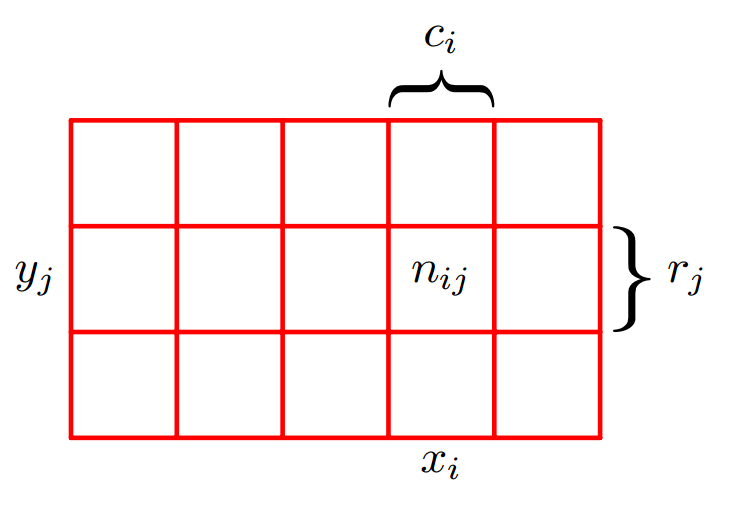
\includegraphics[width=8cm]{Figure1-10.png}}
	\end{figure}
	
	为了推到这两个概率的准则,我们来考虑一个如图1.10所示的更一般的例子,包含两个随机变量\textit{X}和\textit{Y},可以当做上面考虑的例子中的箱子和水果变量。我们假设\textit{X}可以取$x_i, i = 1, \dots, M$的任意值,\textit{Y}可以取值为$y_j, j = 1, \dots, L$。我们考虑变量\textit{X}和\textit{Y}的\textit{N}次抽样试验,用$n_{ij}$表示试验结果为$X = x_i$和$Y = y_j$的试验,用$c_i$表示\textit{X}取值$x_i$的试验次数,$r_j$表示\textit{Y}取值$y_j$的次数。
	
	\textit{X}取值为$x_i$和\textit{Y}取值为$y_j$的概率写为$p(X = x_i, Y = y_j)$,称为$X = x_i$和$Y = y_j$联合概率。由落入单元$i,j$的点的个数占总的个数分数给出,因此
	
	\begin{equation}
	p(X = x_i, Y = y_j) = \frac{n_{ij}}{N}
	\end{equation}
	
	这里隐含考虑$N \to \infty$。类似地,不考虑\textit{Y}时,$X$取值为$x_i$的概率写作$p(X = x_i)$,由落在第\textit{i}列的点的总个数的分数给出,因此
	
	\begin{equation}
	p(X = x_i) = \frac{c_i}{N}
	\end{equation}
	
	因为图1.10中,第i列里面的实例的个数是所有的在这列上的点的实例的个数之和,所以我们得到$c_i = \sigma_j n_{ij}$,因而由(1.5)和(1.6)可以得到
	\begin{equation}
	p(X  = x_i) = \sum_{j = 1}^{L} p(X = x_i, Y = y_j)
	\end{equation}
	
	表示概率的求和准则。注意有时候$p(X = x_i)$称为边缘概率(\textit{marginal}),因为这是通过边缘化或者对另外一个变量的求和得到的,在这个例子中是\textit{Y}。
	
	如果我们只考虑$X = x_i$的实例,对于$Y = y_j$的实例的分数表示为
	\begin{equation}
	p(Y = y_j \mid X = x_i) = \frac{n_{ij}}{c_i}
	\end{equation}
	
	从式子(1.5)(1.6)和(1.8)可以推到出下面的关系
	\begin{equation}
	\begin{aligned}
	p(X = x_i, Y = y_j) & = \frac{n_{ij}}{N} = \frac{n_{ij}}{c_i} \cdot \frac{c_i}{N}\\
	& = p(Y = y_j | X = x_i)p(X = x_i)
	\end{aligned}
	\end{equation}
	
	这个是概率的乘法准则。
	
	目前我们已经谨慎地区分了随机变量(如在水果例子中的\textit{B})和随机变量取值(如\textit{r}表示箱子是红色的)的不同。因此\textit{B}取值\textit{r}的概率表示为$p(B = r)$。尽管这可以避免二义性,但是这会导致比较笨重的标识,在很多情况下,我们并不需要这种迂腐。替代地,我们可以简单地用$p(B)$来表示随机变量\textit{B}的分布,用$p(r)$表示分布的取值\textit{r}的估计,这从上下文可以得到清晰的解析。
	
	通过这种更加简洁的表示,我们用下面的形式来表示这两个基本准则
	
	{\color{red}{概率的准则}}
	
	\textbf{加法准则}
			\begin{equation}
			 p(X) = \sum_Y p(X,Y)
			\end{equation}
	
	\textbf{乘法准则}
			\begin{equation}
			 p(X,Y) = p(Y|X)p(X)
			\end{equation} 

	这里的$p(X, Y)$是联合概率,表示为\textit{X}和\textit{Y}的概率。同样地,$p(Y|X)$是条件概率,表示给定\textit{X}条件下\textit{Y}的概率。其中$p(X)$是边缘分布,仅是\textit{X}的概率。这两个简单的准则形成了概率体系的基础,我们也会在整本书里面使用到。
	
	从乘法准则中可以得到对称属性$p(X, Y) = p(Y, X)$,我们可以得到下面的条件概率关系
	
	\begin{equation}
	p(Y|X) = \frac{p(X|Y)p(Y)}{p(X)}
	\end{equation}
	
	我们称为贝叶斯定理(\textit{Bayes' theorem}),其在模式识别和机器学习中起到核心作用。使用求和准则,贝叶斯定理的分母可以根据出现在分子的项表达
	
	\begin{equation}
	p(X) = \sum_Y p(X|Y)p(Y).
	\end{equation}
	
	我们可以将贝叶斯定理的分母当做标准化常数,需要确保在(1.12)左边对于Y的所有的值的条件概率和为1.
	
	\begin{figure}[t]
		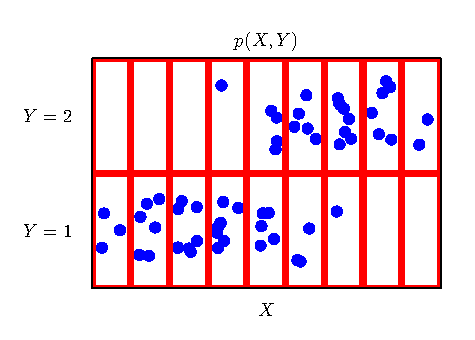
\includegraphics[width=8cm]{Figure1-11a.eps}
		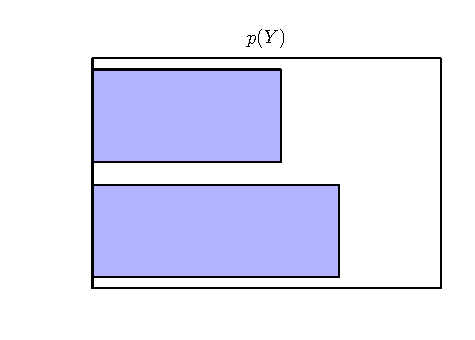
\includegraphics[width=8cm]{Figure1-11b.eps}
		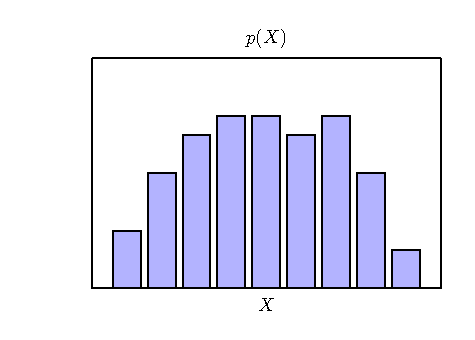
\includegraphics[width=8cm]{Figure1-11c.eps}
		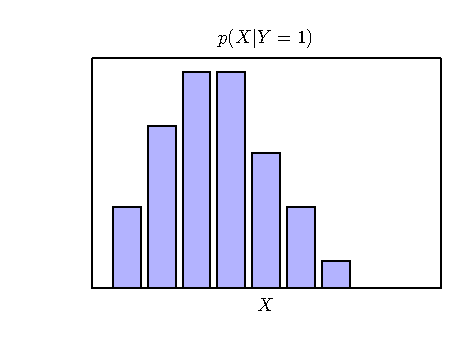
\includegraphics[width=8cm]{Figure1-11d.eps}
		\caption{图例是两个变量的分布\textit{X}和\textit{Y},其中\textit{X}具有9个可能的取值,Y具有两个可能的取值。左上角的图显示了60个点的样本,是这两个随机变量的联合概率分布。剩下的图是是显示了边缘分布$p(X)$和$p(Y)$的直方图估计,和条件分布$p(X|Y = 1)$对应的左上角的图中的底部}
	\end{figure}
	
	在图1.11中,我们可以看到两个变量的联合分布的一个简单例子,描述边缘分布和条件分布的概念。在图的左上角中,是一个N = 60数据点的有限样本得到的联合分布图。右上角是对于Y的每个值得到的部分数据点的柱状图。从概率的定义得到,这个比例等于对应的当极限$N \to \infty$时候的概率$p(Y)$。我们可以看到柱状图作为一个简单的方式,对一个有限点的概率分布建模。从给定的数据对分布进行建模在统计模式识别中占核心地位,我们也会在书中详细地介绍。图1.11中剩下的两个图是用柱状图估计对应的$p(X)$和$p(X|Y = 1)$。
	
	我们现在回到我们的水果箱子的例子。现在我们再次明确随机变量和他们的实例之间的区别。我们看到选择红色或者蓝色箱子的概率分别为
	
	\begin{equation}
	p(B = r) = 4/10
	\end{equation}
	\begin{equation}
	p(B = b) = 6/10
	\end{equation}
	
	这两个概率满足$p(B = r) + p(B = b) = 1$。
	
	现在我们假设我们随机挑选一个箱子,是蓝色箱子。接着选择一个苹果的概率仅仅是在蓝箱子中的苹果的比例为3/4,因此得到$p(F = a| B = b) = 3/4$,事实上,在给定选中的箱子的条件下,我们可以得到所有的四个条件概率
	
	\begin{equation}
	p(F = a|B = r) = 1/4
	\end{equation}
	\begin{equation}
	p(F = o|B = r) = 3/4
	\end{equation}
	\begin{equation}
	p(F = a|B = b) = 3/4
	\end{equation}
	\begin{equation}
	p(F = o|B = b) = 1/4
	\end{equation}
	
	注意到他们的概率是归一化的,因此有
	
	\begin{equation}
	p(F = a|B = r) + p(F = o| B = r) = 1
	\end{equation}
	同样的能得到
	\begin{equation}
	p(F = a|B = b) + p(F = o|B = b) = 1
	\end{equation}
	
	我们现在用乘法公式来估计选择一个苹果的整体的概率
	
	\begin{equation}
	\begin{aligned}
	p(F = a) & = p(F = a|B = r)p(B = r) +p(F = a|B = b)p(B = b)\\
			 & = \frac{1}{4} \times \frac{4}{10} + \frac{3}{4} \times \frac{6}{10}
	\end{aligned}
	\end{equation}
	
	利用加法准则,我们可以得到$p(F = o) = 1 - 11/20 = 9/20$。
	
	假设我们知道已经选择了的一个水果是橘子,那么我们想知道这个橘子是从哪个箱子选出来的。尽管式子(1.16)-(1.19)给出了再给定箱子标识条件下水果的概率,但是我们需要估计给定水果标识的条件下箱子的概率分布。我们可以使用贝叶斯定理反转这个条件概率来解决这个问题
	
	\begin{equation}
	p(B = r|F = o) = \frac{p(F = o|B = r)p(B = r)}{p(F = o)} = \frac{3}{4} \times \frac{4}{10} \times \frac{20}{9}= \frac{2}{3}.
	\end{equation}
	
	根据加法准则,我们可以得到$p(B = b|F = o) = 1 -2/3 = 1/3$。
	
	下面我们提供了贝叶斯定理的一个重要解析。如果我们在知道选择的水果的标识之前,想知道选择了那个箱子,我们可以得到的最完整的的信息就是概率$p(B)$。我们称这个概率为先验概率(\textit{prior probability}),因为这个概率是在我们知道水果的标识之前知道的。一旦我们知道选中的水果是橘子,我们可以用贝叶斯定理来计算概率$p(B|F)$,我们称为后验概率(\textit{posterior probability}),因为这个概率是在我们已经观察\textit{F}后得到的概率。注意到在这个例子中,选择红色箱子的先验概率是4/10,因此相对红色箱子而言,我们更可能选择蓝色箱子。然而我们一旦观察到选择的水果的种类是橘子,我们会发现选择红色箱子的后验概率是2/3,因此实际上我们更可能会选择红色箱子。据我们的直觉所知,在红色箱子中的橘子的比例比蓝色箱子中的橘子比例更大,因而观察得到一个水果的种类是橘子的信息提供了偏向红色箱子的重要证据。实际上,证据表明,先验的比重使得更有可能选择红色箱子而不是蓝色。
	
	最后,我们注意到,当X和Y是相互独立时,两个随机变量的联合概率分解为边缘概率的乘积$p(X, Y) = p(X)p(Y)$。根据乘法准则,我们发现$p(Y|X) = p(Y)$,从而给定\textit{X}条件下\textit{Y}的概率是和\textit{X}相互独立的,例如,在我们的水果箱子例子中,如果箱子包含相同比例的苹果和橘子,有$p(F|B) = p(F)$,因此我们可以说选中一个苹果的概率和选择哪个箱子无关。
	
\subsection{概率密度}

	考虑了定义在离散事件上的概率,我们现在来考虑连续变量的概率。我们会进行相对正式的讨论。如果一个实数变量\textit{x}落在区间$(x, x + \delta x)$的概率给出为$p(x)\delta x, \delta x \to 0$,我们就可以称$p(x)$为\textit{x}的概率密度,如图1.12所示。\textit{x}在区间(a,b)上的的概率为
	
	\begin{equation}
	p(x \in (a,b)) = \int_{a}^{b} p(x) d(x).
	\end{equation}
	
	\begin{figure}[t]
		\parbox{.4\textwidth}{\caption{离散型随机变量的概率概念可以扩展为连续型变量的盖里密度$p(x)$,其中x在区间$(x, x + \delta x)$的概率给出为$p(x)\delta x, \delta x \to 0$,概率密度可以用累积分布函数$P(x)$的导数来表达}}
		\parbox{.5\textwidth}{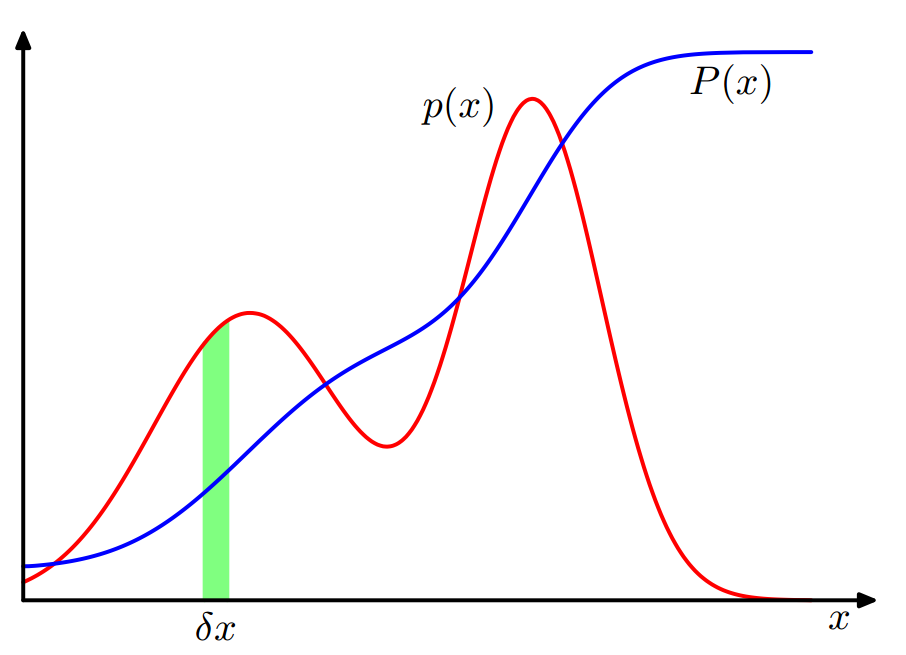
\includegraphics[width=8cm]{Figure1-12.png}}
	\end{figure}
	
	因为概率是非负的,并且x值必须位于实数轴上,因此概率密度$p(x)$必须满足两个条件
	
	\begin{equation}
	p(x) \geq 0
	\end{equation}
	\begin{equation}
	\int_{- \infty}^{\infty} p(x) d(x) = 1.
	\end{equation}
	
	在变量的非线性变化情况下,由于Jacobian因子的原因,概率密度的改变和简单的函数不一样。例如,我们考虑单变量的改变$x = g(y)$,因而函数$f(x)$变为$\tilde{f}(y) = f(g(y))$。现在我们来考虑概率密度$p_x(x)$,对应的新变量\textit{y}的的密度为$p_y(y)$,能够充分表明$p_x(x)$和$p_y(y)$是不同的密度。观察值落入范围$(x, x + \delta x)$可以转换为范围$(y, y + \delta y)$,其中$p_x(x) \simeq p_y(y) \delta y$,因此
	
	\begin{equation}
	\begin{aligned}
	p_y(y) & = p_x(x) \mid \frac{dx}{dy} \mid\\
		   & = p_x(g(y)) \mid g' (y) \mid
	\end{aligned}
	\end{equation}
	
	这个性质的一个结果是概率密度的最大值与所选的变量相互独立。
	
	变量\textit{x}在区间$(- \infty, z)$的概率可以由累积分布函数定义为
	
	\begin{equation}
	P(z) = \int_{- \infty}^{z} p(x)dx.
	\end{equation}
	
	式子满足$P'(x) = p(x)$,如图1.12所示.
	
	如果有几个连续的变量$x_1, \dots, x_D$,用集合方式表示为向量$\mathbf{x}$,接着我们可以定义联合概率密度为$p(\mathbf{x}) = p(x_1, \dots, x_D)$。$\mathbf{x}$落在包含$\mathbf{x}$的无穷小量$\delta \mathbf{x}$的概率为$p(\mathbf{x}) \delta \mathbf{x}$。这种多变量概率密度必须满足
	
	\begin{equation}
	p(\mathbf{x}) \geq 0
	\end{equation}
	\begin{equation}
	\int p(\mathbf{x}) dx = 1
	\end{equation}
	
	其中积分取值为$\mathbf{x}$整个向量空间。我们同样可以在离散和连续的变量结合之上考虑联合概率分布。
	
	注意到如果$\mathbf{x}$是离散变量时,$p(x)$有时候也称为\textbf{概率密度函数}(\textit{probability mass function}),因为它可以被视为x可取值的“概率密度”的集合。
	
	概率的加法和乘法准则,和贝叶斯定理一样,同样适用于概率密度,或者是离散和连续变量的结合。例如,如果\textit{x}和\textit{y}是两个实数变量,那么加法和乘法准则可以写为
	
	\begin{equation}
	p(x) = \int p(x, y) dy
	\end{equation}
	\begin{equation}
	p(x, y) = p(y|x)p(x).
	\end{equation}
	
	连续变量的加法和乘法准则的一个正规的证明需要数学中的一个分支,称为\textbf{测量理论}(\textit{measure theory}),超过了本书的范围。公式的验证可以通过非正式的方法来看,通过将变量划分为宽度为$\Delta$区间,然后只考虑在这些区间上的离散的概率分布。取当极限$\Delta \to 0$时候的各个区间的和就可以得到期望的结果。
	
%1.2.2 Expectations and covariances
\subsection{期望和方差}
	概率的一个最重要的操作是找到函数的加权平均值,某些函数$f(x)$在概率分布$p(x)$下的均值称为$f(x)$期望,表示为$\mathbb{E}[f]$。对于离散分布,表示为
	
	\begin{equation}
	\mathbb{E}[f] = \sum_x p(x)f(x)
	\end{equation}
	
	因此均值是不同\textit{x}值的相关概率的加权。在连续型变量中,期望表达的是一个整数关于对应的概率密度
	
	\begin{equation}
	\mathbb{E}(f) = \int p(x) f(x) dx.
	\end{equation}
	
	在每个例子中,如果我们给定N个从概率分布和概率密度中提取的点,期望就可以近似为这些点的有限和
	
	\begin{equation}
	\mathbb{E}(f) \simeq \frac{1}{N} \sum_{n = 1}^{N} f(x_n).
	\end{equation}
	
	我们在后面第11章讨论的样例方法时候会扩展这个结果。当$N \to \infty$时,式子(1.35)这个近似值趋近真值。
	
	有时候我们会考虑函数多个变量的期望,我们会使用下标来表示哪个变量要来均值,例如
	
	\begin{equation}
	\mathbb{E}_x[f(x,y)]
	\end{equation}
	
	表示函数$f(x, y)$相对于\textit{x}分布的均值,注意到$\mathbb{E}_x [f(x, y)]$是关于\textit{y}的函数。
	
	我们可以考虑相对于条件分布的条件期望,因此
	
	\begin{equation}
	\mathbb{E}_x [f|y] = \sum_x p(x|y)f(x)
	\end{equation}
	
	对于连续变量有类似的定义。
	
	函数$f(x)$的\textbf{方差}(\textit{variance})定义为
	
	\begin{equation}
	\mathrm{var}[f] = \mathbb{E} [(f(x) - \mathbb{E}[f(x)])^2]
	\end{equation}
	
	提供了一种方法来测量在函数$f(x)$中有多少值在均值$\mathbb{E}[f(x)]$周围波动。对公式的平方展开,我们可以看到方差可以写为$f(x)$和$f(x)^2$的期望
	
	\begin{equation}
	\mathrm{var}[f] = \mathbb{E} [f(x)^2] - \mathbb{E}[f(x)]^2.
	\end{equation}
	
	特别的,当我们考虑变量\textit{x}自身时,可以得到
	
	\begin{equation}
	\mathrm{var}[x] = \mathbb{E}[x^2] - \mathbb{E}[x]^2.
	\end{equation}
	
	对于两个随机变量\textit{x}和\textit{y},\textbf{协方差}(\textit{covariance})定义为
	
	\begin{equation}
	\begin{aligned}
	\mathrm{var}[x, y] & = \mathbb{E}_{x,y}[\{x - \mathbb{E}[x]\}\{ y - \mathbb{E}[y] \}]\\
					   & = \mathbb{E}_{x,y}[xy] - \mathbb{E}[x]\mathbb{E}[y]
	\end{aligned}
	\end{equation}
	
	表达了\textit{x}和\textit{y}一起的变化。如果x和y是相互独立的,那么他们没有方差。
	
	在两个向量的随机变量\textbf{x}和\textbf{y}的例子中,协方差是一个矩阵
	
	\begin{equation}
	\begin{aligned}
	\mathrm{var}[\textbf{x}, \textbf{y}] & = \mathbb{E}_{\textbf{x},\textbf{y}}[\{\textbf{x} - \mathbb{E}[\textbf{x}]\}\{ \textbf{y}^T - \mathbb{E}[\textbf{y}^T] \}]\\
	& = \mathbb{E}_{\textbf{x},\textbf{y}}[\textbf{xy}^T] - \mathbb{E}[\textbf{x}] \mathbb{E}[\textbf{y}^T]
	\end{aligned}
	\end{equation}
	
	如果我们考虑向量\textbf{x}和自身的协方差,我们可以使用简单的符号来表示$\mathrm{var}[\textbf{x}] \equiv \mathrm{var}[\textbf{x},\textbf{x}]$.
	
\subsection{贝叶斯概率}
	 目前在这章中,我们已经在随机重复事件的频率上观察概率。我们将会将这当做经典的或者频繁的概率解析。现在我们转向更一般的贝叶斯视角,概率会提供一种不确定性的量化。
	 
	 考虑一个不确定事件,例如月亮是否在太阳的轨道上,或者两极的冰川将会在本世纪末消失。这些事件不是许多事件的重复,能和前面我们讨论的水果箱子问题一样可以定义一个概率的概念。尽管如此,我们通常也会有一些想法,如我们可以考虑冰川融化的速度。如果我们获取新的证据,例如从地球观测人造卫星上收集地球的诊断信息,我们或许可以修订对于冰川消失速度的选择。我们的这种评估方案会影响我们所采取的行动,例如一个扩展是,我们尽力去减少温室气体的排放。在这种情况下,我就可以去量化对于不确定性的表达,并用新的证据来精确地修订不确定性,接下来最后也可以采取最优的行动或决策。这可以通过优雅的,并很一般的概率贝叶斯解析来实现。
	 
	 然而使用概率来表达不确定性并不是一个专业的选择,但在进行合理连贯性推理的时候我们必然会遵循这种常识。例如Cox(1946)表明如果数值型值用来信念度时,使用一个定理集合来对这种信念的常识属性进行编码会导致唯一的一套信念操作度规则集合,等价于概率的加法和乘法准则。这里提供了概率理论可以被视为包含不确定性的布尔逻辑的扩展的严格证明(Jaynes,2003)。很多其他的作者也提出了关于不确定性应该满足的的测量方法的不同属性和公理集合(Ramsey, 1931; Good, 1950; Savage, 1961; deFinetti, 1970; Lindley, 1982)。在每个例子中,根据概率的规则进行了精确的数值型量化。因此涉及到这种量化自然被称为贝叶斯概率。
	 
	 在模式识别中,有很多通用的概率标识是很有用的。考虑1.1节的多项式曲线拟合的例子,将概率中频繁的标识应用到观测变量$t_n$的随机值是合理的。然而,我们想处理和量化在模型参数\textbf{w}的近似选择周围的不确定性。我们可以看到,从贝叶斯的视角,我们可以使用贝叶斯理论的工具去描述在模型中如\textbf{x}的不确定性,或者模型自身的选择。
	 
	 贝叶斯现在有了新的意义。我们回忆在水果箱子的例子中,水果标识的观察值为断言选择箱子是红色的概率的提供了相关信息。在那个例子中,贝叶斯定理通过合并观测数据提供的证据来将先验概率转化为后验概率。我们会在后面看到详细的过程,我们可以采用相同的方法对量化进行推理,如在多项式曲线拟的例子中的参数\textbf{w}。在观察数据之前,我们对在先验概率分布$p(x)$中的\textbf{w}做出假设。通过条件概率来对观测数据$\mathcal{D} = \{ t_1, \dots, t_N \}$的影响进行表达,我们在后面的1.2.5节中可以看到如何进行明确表达。贝叶斯理论,可以具有下面的形式
	 
	 \begin{equation}
	 p(\textbf{w} | \mathcal{D}) = \frac{p(\mathcal{D} | \textbf{w})p(\textbf{w})}{p(\mathcal{D})}
	 \end{equation}
	 
	 这允许我们在后验概率$p(\textbf{w}|\mathcal{D})$的形式下观察$\mathcal{D}$之前估计在\textbf{w}中的不确定性。
	 
	 在贝叶斯定理右边的量化值$p(\mathcal{D} | \textbf{w})$可以通过观测数据$\mathcal{D}$进行估计,可以被当做参数向量\textbf{w}的一个函数,在这个例子中称为\textbf{似然函数}((\textit{likehood function})表达了观测数据集对于参数向量\textbf{w}的不同设置的的可能性。注意到似然不是\textbf{w}的概率分布,对于\textbf{w}的整体是不等于1的。
	 
	 给出了似然的定义,我们可以用文字来叙述贝叶斯定理
	 
	 \begin{equation}
	 \mathrm{posterior \propto likelihood \times prior}
	 \end{equation}
	 
	 其中所有的量化值都是\textbf{w}的函数。在式子(1.43)中的分母是常数,确保了再左边的后验概率是有效的概率密度,并且和为1.我们相对于\textbf{w}公式(1.43)两端进行积分,我们可以用贝叶斯定理的后验分布和似然函数来表达分母
	 
	 \begin{equation}
	 p(\mathcal{D}) = \int p(\mathcal{D} | \textbf{w}) p(\textbf{w}) d\textbf{w}.
	 \end{equation}
	 
	 在贝叶斯学派和频率学派中,似然函数$p(\mathcal{D} | \textbf{w})$起到了核心作用。然而,在两种方法使用的基础是不一样的。在频率学派设置中,\textbf{w}是一个固定的参数,其由一些估计量来确定,在估计中的误差线是通过考虑可能数据集$\mathcal{D}$的分布来获得。相比之下,从贝叶斯的视角之下,只存在单独的数据集$\mathcal{D}$(称为真实的观测值),在参数中的不确定性是通过\textbf{w}的概率分布来表示。
	 
	 广泛使用频率学派估计量的是\textbf{最大似然}(\textit{maximum likelihood}),其中\textbf{w}值被设置为当似然函数$p(\mathcal{D} | \textbf{w})$最大时的值。这对应于选择\textbf{w}使得观测值的概率取值最大。在机器学习的文献中,似然函数的对数的相反数称为\textbf{误差函数}(\textit{error function})。因为对数的相反数是单调递减的,因此最大化似然函数就等价于最小化误差函数。
	 
	 确定频率学派的误差线的一种方法是\textbf{自助}(\textit{bootstrap})(Efron, 1979; Hastie et al., 2001),其中多个数据集通过下面的方式来产生。假设我们原始数据集包含\textit{N}个点$\textbf{X} = \{ \textbf{x}_1, \dots, \textbf{x}_N \}$。我们可以通过从数据集\textbf{X}随机选取\textit{N}个点来产生一个新的数据集$\textbf{X}_B$,其中在$\textbf{X}$中有些点在$\textbf{X}_B$中是重复的,反之,在$\textbf{X}$中的有些点不会出现在$\textbf{X}_B$中。这个过程可以重复\textit{L}次产生\textit{L}个数据集,每个数据集的长度为\textit{N},并且每个数据集都是从原数据集\textbf{X}中抽样得到。参数估计的统计精度可以通过在不同自助数据集中的预测变化来得估计。
	 
	 使用贝叶斯观点的一个优点是先验知识可以很自然就提出了。例如,假设正常的银币掷三次,每次都是正面朝上,一个比较典型的最大似然估计是正面朝上的概率是1,意味着在后面掷银币都会得到正面朝上。相反的,在贝叶斯方法中,任何合理的先验后会使得很少出现极端的结论。
	 
	 这里有很多关于频率学派和贝叶斯学派的优点的论战,这对于只有频率学派或者只有贝叶斯学派的视角并没有意义。例如,对贝叶斯的一个批评是先验分布的选择是基于数学方便性的选择,而不是先验信念的反射。通过他们对选择先验的依赖性导致结论的主观性似乎是困难的来源。
	 
	 减少对先验选择的依赖性是\textbf{无信息先验}(noninformative priors)的一个动机。然而,当对比不同模型时,这会产生很多困难,特别是基于对先验糟糕选择的贝叶斯方法可能会给出置信度很高的糟糕结果。频率学派评估方法提供了防止这种问题的一些防护,和一些技术如交叉验证在模型比较仍然很有用。
	 
	 这本书主要强调贝叶斯观点,反映了过去的几年里贝叶斯方法在实践中重要性的巨大提升。我们也会讨论频率学派的一些有用概念。
	 
	 尽管贝叶斯框架起源于18世纪,但是贝叶斯方法的实际应用经历了很长一段时间,是由于通过整个贝叶斯过程来实施的困难的限制,尤其是边缘化(求和或者整体)整个参数空间的需要,我们为了进行决策或者比较不同模型时就会需要到这个过程。随着抽样方法的发展,马尔科夫链蒙特卡洛戏剧性提高了地在计算机上的计算的速度和内存空间能力,打开了贝叶斯技术在实践中使用的大门,其问题的范围令人钦佩。蒙特卡洛方法很灵活,并且应用模型很广泛。然而,它们是计算集中型的,主要在小规模的问题中使用。
	 
	 最近,一些高效的确定性近似方案如变分贝叶斯和期望传播已经发展起来(在第10章会讨论)。这些对抽样方法进行了补充,并且允许贝叶斯技术在大规模的应用中使用(Blei et al., 2003)。
	 
\subsection{高斯分布}
	 整个第二章的是学习各种概率分布和他们的主要性质。这里方便介绍一个最重要的连续变量概率分布,称为\textbf{正态分布}(\textit{normal distribution})或者\textbf{高斯分布}(\textit{Guassian distribution}),我们会在本章剩余部分来介绍这个分布的使用,并且会贯穿整本书的很多内容。
	 
	 对于单实数变量\textit{x},高斯分布可以表示为
	 
	 \begin{equation}
	 \mathcal{N}(x | \mu, \sigma^2) = \frac{1}{(2 \pi \sigma^2)^(1/2)} \mathrm{exp}\{- \frac{1}{2 \sigma^2}(x - \mu)^2\}
	 \end{equation}

	公式由两个参数确定,一个是均值$\mu$,一个是方差$\sigma^2$。方差的开方$\sigma$称为\textbf{标准差}(\textit{standard deviation}),方差的倒数$\beta = 1/\sigma^2$称为\textbf{精确度}(\textit{precision}),我们将会简要地看到这些项的动机。图1.13显示了高斯分布的点图。
	
	\begin{figure}[b]
		\parbox{.4\textwidth}{\caption{ 单变量高斯分布显示了均值$\mu$和标准差$\sigma$ }}
		\parbox{.5\textwidth}{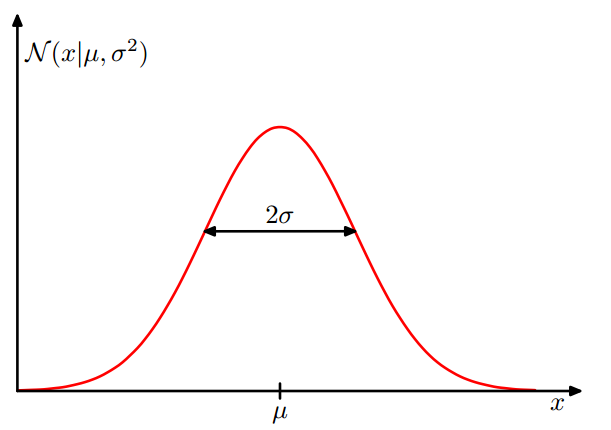
\includegraphics[width=8cm]{Figure1-13.png}}
	\end{figure}
	
	从式子(1.46)中我们可以看到高斯分布满足
	
	\begin{equation}
	\mathcal{N}(x | \mu, \sigma^2) > 0.
	\end{equation}
	
	这也直接看出高斯是标准化的,因此
	
	\begin{equation}
	\int_{- \infty}^{\infty} \mathcal{N}(x | \mu, \sigma^2) dx = 1.
	\end{equation}
	
	因此公式(1.46)满足概率密度的两个要求。
	
	我们可以容易地找到\textit{x}的函数在高斯分布下的期望,特别地,\textit{x}的平均值为
	
	\begin{equation}
	\mathbb{E}[x] = \int_{- \infty}^{\infty} \mathcal{N}(x | \mu, \sigma^2) x dx = \mu.
	\end{equation}
	
	因为参数$\mu$反映的是\textit{x}在分布下的平均值,称为均值。同样的,对于二阶矩
	
	\begin{equation}
	\mathbb{E}[x^2] = \int_{- \infty}^{\infty} \mathcal{N}(x | \mu, \sigma^2) x^2 dx = \mu^2 + \sigma^2.
	\end{equation}
	
	从式子(1.49)和(1.50)可以得到\textit{x}的方差为
	
	\begin{equation}
	\mathrm{var}[x] = \mathbb{E}[x^2] - \mathbb{E}[x]^2 = \sigma^2
	\end{equation}
	
	因此$\sigma^2$称为方差变量。分布的最大值称为模式。对于高斯分布,模式与均值具有一致性。
	
	我们也感兴趣定义在D维向量随机变量\textbf{x}上的高斯分布,可以得到
	
	\begin{equation}
	\mathcal{N}( \mathbf{x}  |  \mathbf{\mu} , \mathbf{ \Sigma }) = \frac{1}{(2\pi)^{D/2}} \frac{1}{ |\mathbf{\Sigma}|^{1/2} }\mathrm{exp} \{ -\frac{1}{2}(\mathbf{ x } - \mathbf{ \mu })^T \mathbf{\Sigma}^{-1}(\mathbf{x} - \mathbf{\mu}) \}
	\end{equation}
	
	\textit{D}维向量$\mathbf{\mu}$称为均值,$D \times D$举证$\mathbf{\Sigma}$称为协方差,$|\mathbf{\Sigma}|$表示$\mathbf{\Sigma}$的行列式。高斯分布的属性会在2.3节中学习,但在这章我们会简单地使用多维高斯分布。
	
	现在假设我们有观察值的一个数据集$\mathsf{x} = (x_1, \dots, x_N)^T$,表示N个标量的观测值。我们使用字体$\mathsf{x}$区分向量值变量$(x_1, \dots, x_D)^T$的一个观测值,表示为\textbf{x}。我们假设观测值是从均值$\mu$和方差$\sigma^2$未知的高斯分布独立地提取出来的,接着我们想通过这些数据集来确定参数。从相同分布中独立提取的数据集称为\textbf{独立同分布}(\textit{independent and identically distributed}),通常简写为 i.i.d。我们已经看到两个独立事件的联合分布通过没个事件的边缘分布的乘积得到。因为我们的数据集$\mathsf{x}$是独立同分布的,因此我们可以由$\mu$和$、sigma^2$来得到数据集的概率形式为
	
	\begin{equation}
	p(\mathsf{x} | \mu, \sigma^2) = \prod_{n = 1}^{N} \mathcal{N}(x_n|\mu, \sigma^2).
	\end{equation}
	
	当公式被看为是关于$\mu$和$\sigma^2$时,这是高斯分布的似然函数,可以通过图1.14的图来解析。
	
	\begin{figure}[t]
		\parbox{.4\textwidth}{\caption{ 高斯分布的似然函数在图中用红色曲线来表示。黑色点表示数据集$\{ x_n \}$,通过式子(1.53)得到的似然函数对应蓝色点值的乘积,最大化似然值包含调整高斯分布的均值和方差使得最大化这个值 }}
		\parbox{.5\textwidth}{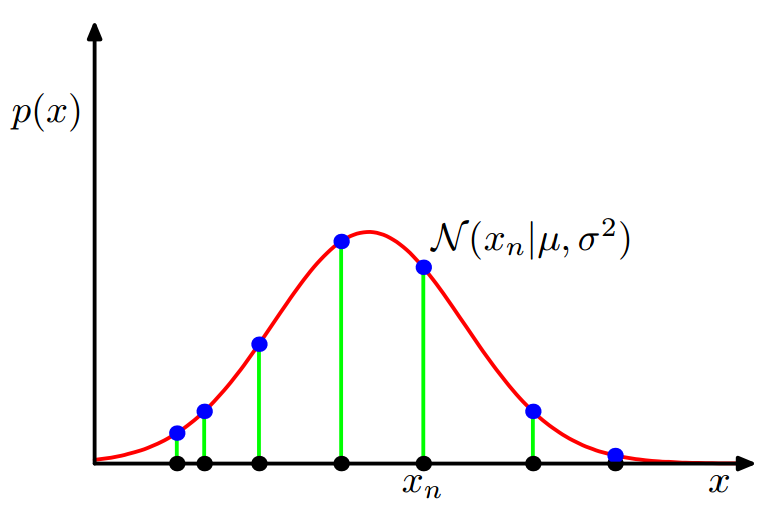
\includegraphics[width=8cm]{Figure1-14.png}}
	\end{figure}
	
	通过观测数据集来确定概率分布参数的一个常用准则是找到参数使得最大化似然函数。这似乎是一个奇怪的准则,从我们前面对概率理论的讨论得到,这似乎很自然地最大化从数据中得到参数的概率,而不是给定参数,最大化数据的概率。事实上,这两种准则是相关联的,正如我们将要讨论的曲线拟合。
	
	现在我们通过最大化似然函数来确定高斯分布中未知参数$\mu$和$\sigma^2$的值。在实际中,最大化似然函数的对数通常更方便。因为对数函数关于参数是单调递增函数,最大化对数里面的函数等价于最大化函数自身。取对数不仅仅是简单的数学分析,也可以数值化,因为很多小概率的乘积会很容易溢出计算机的数值精度,这可以通过计算概率的对数的和来代替。从式子(1.46)和(1.53)可以得到似然函数的形式为
	
	\begin{equation}
	\ln p(\mathsf{x} | \mu, \sigma^2) = -\frac{1}{2 \sigma^2} \sum_{n = 1}^{N} (x_n - \mu)^2 - \frac{N}{2}\ln \sigma^2 - \frac{N}{2} \ln(2 \pi).
	\end{equation}
	
	关于$\mu$最大化式子(1.54),我们可以通过公式得到最大似然结果
	
	\begin{equation}
	\mu_{ML} = \frac{1}{N} \sum_{n = 1}^{N} x_n
	\end{equation}
	
	称为样本均值,也就是观测值$\{ x_n\}$的均值。同样的,最大化关于$\sigma^2$的式子(1.54),我们可以获得关于方差的最大似然结果的形式
	
	\begin{equation}
	\sigma_{ML}^2 = \frac{1}{N} \sum_{n = 1}^{N}(x_n - \mu_{ML})^2
	\end{equation}
	
	称为对应于样本均值$\mu_{ML}$的样本方差。注意到我们是要最大化关于$\mu$和$\sigma^2$的式子(1.54)。但在高斯分布的例子中,从$\sigma^2$中分离出$\mu$,就可以先估计式子(1.55),接着使用这个结果来估计(1.56)。
	
	在本章的后面和后续的章节里,我们会强调最大似然估计法的局限性,在单变量高斯分布的最大似然估计参数设置中,这里我们给出我们结果的问题提示。特别的,我们会展示最大似然法整体上低估了分布的变量。这个例子的现象称为\textbf{偏差}(\textit{bias}),和过拟合相关的问题在多项式曲线拟合背景下会遇到。我们首先会注意到最大似然结果$\mu$和$\sigma_{ML}^2$是关于数据集的值$x_1, \dots, x_N$的函数。考虑关于数据集量化的期望,这些数据来自于参数为$\mu$和$\sigma_2$的高斯分布。直接得到
	
	\begin{equation}
	\mathcal{E}[\mu_{ML}] = \mu
	\end{equation}
	\begin{equation}
	\mathcal{E}[\sigma_{ML}^2] = (\frac{N - 1}{N}) \sigma^2
	\end{equation}
	
	因此通常最大似然估计会得到正确的均值,但会低估正确的方差,因子为$(N - 1)/N$。在这个结果后的直觉可以从图1.15中得到。
	
	\begin{figure}[t]
		\parbox{.5\textwidth}{\caption{  如图所示,在使用最大似然去确定高斯分布的方差时产生的偏差。绿色曲线表示从数据中得到的正确的高斯分布,三条红色的曲线是通过拟合三个数据集得到的,每条曲线包含两个数据点,用蓝色表示,使用最大似然结果(1.55)和(1.56)。平均三个数据集,得到的均值是正确的,但是方差整体上低估了,因为测量的结果是和样本均值相关而不是和正真的均值相关 }}
		\parbox{.5\textwidth}{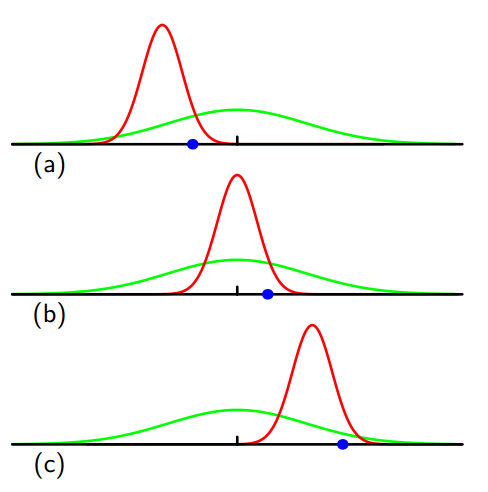
\includegraphics[width=8cm]{Figure1-15.png}}
	\end{figure}
	
	从式子(1.58)中得到下面对于方差参数估计是无偏的
	
	\begin{equation}
	\tilde{\sigma}^2 = \frac{N}{N - 1}\sigma_{ML}^2 = \frac{1}{N - 1} \sum_{n - 1}^{N}(x_n - \mu_{ML})^2.
	\end{equation}
	
	在10.1.3节中,我们会看到,当使用贝叶斯方法时,结果是如何自动得到的。
	
	注意到当数据点的数量N增加时,最大似然结果的偏差会变得越小,并且在极限$N \to \infty$时最大似然的结果方差会等于正真产生这些数据的分布的方差。在实际中,除了小N,这种偏差并不是大问题。然而,在整本书中,我们对有很多参数的复杂模型感兴趣,对于和最大似然相关的偏差问题会变得很严重。事实上,正如我们所看到的,最大似然中的偏差问题位于过拟合的基础上,过拟合问题在前面的多项式曲线拟合中遇到。
	
\subsection{曲线拟合}
	我们已经看到多项式曲线拟合可以表达为误差的最小化。现在我们回到曲线拟合的例子,然后用概率的视角来看,从而思考误差函数和归一化,也将我们带入全贝叶斯处理。
	
	曲线拟合问题的目标是可以对给定的新的输入变量x,做出预测目标变量t,基于一个包含N个输入值$\mathsf{x} = (x_1, \dots, x_N)^T$的训练数据集,对应的目标值为$\mathsf{t} = (t_1, \dots, t_N)^T$。我们可以使用概率分布来表达我们的不确定性。这样一来,我们可以假设给定的值\textit{x},对应的值\textit{t}具有均值为$y(x, \textbf{w})$的高斯分布,其中均值是来自于公式(1.1)给出的多项式曲线。因此我们能得到
	
	\begin{equation}
	p(t |x, \textbf{w}, \beta) = \mathcal{N}(t| y(x,\textbf{w}, \beta^{-1}))
	\end{equation}

	对于连续的标识会在后面的章节来介绍,我们已经定义了精确度参数$\beta$,对应到分布方差的逆。在图1.16中会示意性地描述。
	
	\begin{figure}[t]
		\parbox{.4\textwidth}{\caption{  图解描述了(1.60)给出的给定\textit{x}时关于\textit{t}的高斯条件分布,其中均值由多项式函数$y(x, \textbf{w})$给出,精确度为$\beta$,对应于方差$\beta^{-1} = \sigma^2$ }}
		\parbox{.5\textwidth}{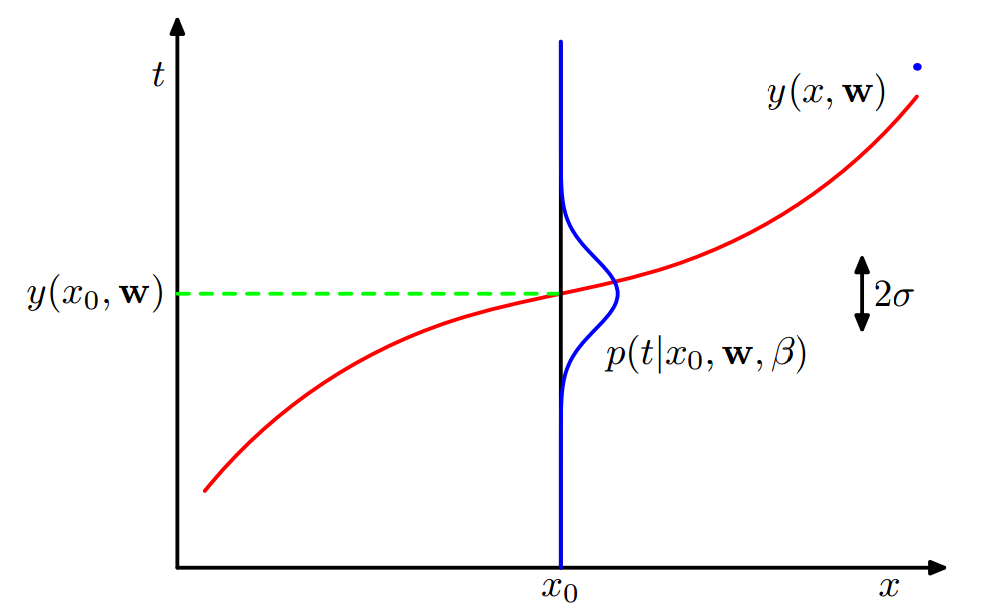
\includegraphics[width=8cm]{Figure1-16.png}}
	\end{figure}
	
	现在我们使用训练数据$\{ \mathsf{x, t} \}$来通过最大似然函数来确定未知参数\textbf{w}和$\beta$的值。假设数据是从分布(1.60)中独立地提取出来的,那么似然函数为
	
	\begin{equation}
	p(\mathsf{t|x}, \textbf{w}, \beta) = \prod_{n = 1}^{N} \mathcal{N}(t_n| y(x_n, \textbf{w}), \beta^{-1}).
	\end{equation}
	
	正如前面我们对简单高斯分布的例子所做的那样,很容易最大化似然函数的对数。由公式(1.46)给出的高斯分布的替代形式,我们得到对数似然函数的形式
	
	\begin{equation}
	\ln p(\mathsf{t|x}, \textbf{w}, \beta) = -\frac{\beta}{2} \sum_{n = 1}^{N} \{ y(x_n, \textbf{w}) - t_n \}^2 + \frac{N}{2}\ln \beta - \frac{N}{2} \ln (2 \pi).
	\end{equation}
	
	考虑确定多项式系数的最大似然结果,可以表示为$\textbf{w}_{ML}$。这可以通过最大化关于w的式子(1.62)。我们可以忽略右边的最后两项,因为它们和\textbf{w}无关。我们也可以注意到用正常数对对数似然函数进行缩放不会改变关于w的最大化值位置。我们可以用1/2来代替$\beta/2$。最后我们并不是最大化对数似然函数,而是最小化等价的负数对数似然函数。因此我们可以看到最大化似然函数等价于最小化(1.2)定义的\textbf{误差平方和函数}(\textit{sum-of-squares error function})来确定\textbf{w}。因此误差平方和函数在假定满足高斯噪声分布下最大化似然函数下提出。
	
	我们也可以使用最大化似然函数来确定高斯条件分布的精度参数$\beta$。最大化关于$\beta$的(1.62)
	
	\begin{equation}
	\frac{1}{\beta_{ML}} = \frac{1}{N} \sum_{n = 1}^{N}\{ y(x_n, \textbf{w}_{ML}) - t_n \}^2
	\end{equation}

	我们首先调整均值来确定参数向量$\textbf{w}_{ML}$,接着使用它确定精度$\beta_{ML}$,和之前的简单高斯分布一样。
	
	已经确定了参数\textbf{w}和$\beta$后,我们可以对于新的值做出决策。因为我们现在有一个概率模型,这可以表示为预测分布,给出了关于t的概率分布,而不是简单的点估计,这可以通过将最大似然参数带入式子(1.60)得到
	
	\begin{equation}
	p(t|x, \textbf{w}_{ML}, \beta_{ML}) = \mathcal{N}(t|y(x, \textbf{w}_ML), \beta_{ML}^{-1})
	\end{equation}
	
	现在让我们来采用更接近贝叶斯方法的步骤来介绍在多项式系数\textbf{w}上的先验分布。简单来说,让我们考虑高斯分布的形式
	
	\begin{equation}
	p(\textbf{w}|\alpha) = \mathcal{N}(\textbf{w}|\textbf{0}, \alpha^{-1}\textbf{I}) = (\frac{\aleph}{2 \pi})^{(M+1)/2} \mathrm{exp}\{ -\frac{\alpha}{2}\textbf{w}^T\textbf{w} \}
	\end{equation}
	
	其中$\alpha$是分布的参数,$M+1$是\textit{M}阶多项式的向量\textbf{w}的元素个数。参数如$\alpha$控制模型分布的参数,称为\textbf{超参数}(\textit{hyperparameters})。使用贝叶斯定理,\textbf{w}的后验分布正比于先验分布和似然函数的乘积。
	
	\begin{equation}
	p(\textbf{w}|\mathsf{x,t},\alpha, \beta) \propto p(\mathsf{t}|\mathsf{x}, w, \beta)p(\textbf{w}|\alpha).
	\end{equation}
	
	现在我们可以确定\textbf{w},找到给定数据条件下最可能的\textbf{w}值,换句话说就是最大化后验分布。这种方法称为\textbf{最大后验概率}(\textit{maximum posterior}),简写为\textit{MAP}。采用(1.66)的负对数,并且结合(1.62)和(1.65),我们可以得到最大的后验概率,通过最小化下面式子
	
	\begin{equation}
	\frac{\beta}{2} \sum_{n = 1}^{N} \{ y(x_n, \textbf{w}) - t_n \}^2 + \frac{\alpha}{2} \textbf{w}^T\textbf{w}
	\end{equation}  
	
	因此我们看到最大化后验分布等价于最小化归一化的误差平方和函数,我们在之前遇到过的(1.4),使用归一化参数为$\lambda = \alpha / \beta$。
	
\subsection{贝叶斯曲线拟合}
	尽管我们已经包含了后验分布$p(\textbf{w}|\alpha)$,但是我们目前还是只进行\textbf{w}的点估计,并没有等于用贝叶斯方法。在全贝叶斯方法里面,我们应该连续地使用概率加法和乘法准则。这要求我们对所有的\textbf{w}值进行积分。这种边缘化位于模式识别贝叶斯方法的核心。
	
	在曲线拟合问题中,我们给出了训练数据$\mathsf{x}$和$\mathsf{t}$,对于一个新测试点\textit{x},我们的目标是预测\textit{t}值。我们因此希望估计预测分布$p(t|x,\mathsf{x},\mathsf{t})$。这里我们假设参数$\alpha$和$\beta$是固定的,并且是已知的。在后面的章节中我们会讨论如何使用贝叶斯方法来推理得到这些参数。
	
	贝叶斯方法仅仅对应于连续使用概率的加法和乘法准则,这允许预测分布可以写为如下形式
	
	\begin{equation}
	p(t|x, \mathsf{x}, \mathsf{t}) = \int p(t| x, \textbf{w}) p(\textbf{w}| \mathsf{x}, \mathsf{t})d\textbf{w}
	\end{equation}
	
	其中$p(t|x, \textbf{w})$可以由(1.60)得到,并且我们忽略$\alpha$和$\beta$之间的依赖性,只是简单地当做符号。这里$p(\textbf{w}|\mathsf{x}, \mathsf{t})$是参数的后验分布,可以通过(1.66)的右端得到。在3.3节中我们可以看到对于这种如曲线拟合的问题,后验分布是一个高斯分布,并且可以同分分析来评估。同样的,对公式(1.68)进行积分也可以分析得到这样的结果,预测分布可以通过高斯分布来得到下面形式
	
	\begin{equation}
	p(t|x, \mathsf{x}, \mathsf{t}) = \mathcal{N}(t|m(x),s^2(x)
	\end{equation}
	
	其中均值和方差可以通过下面式子得到
	
	\begin{equation}
	m(x) = \beta \phi (x)^T \textbf{S} \sum_{n = 1}^{N} \phi (x_n) t_n
	\end{equation}
	\begin{equation}
	s^2(x) = \beta^{-1} + \phi (x)^T \textbf{S} \phi (x).
	\end{equation}
	
	这里的矩阵\textbf{S}为
	
	\begin{equation}
	\textbf{S}^{-1} = \alpha \textbf{I} + \beta \sum_{n = 1}^{N} \phi (x_n) \phi (x)^T
	\end{equation}
	
	式子中的\textbf{I}为单位矩阵,我们定义向量$\phi(x)$ 为$\phi (x) = x^i, i = 0, \dots, M$。
	
	我们看到预测分布的均值和方差是依赖于\textit{x}的。式子(1.71)中的首项表达了预测值\textit{t}的不确定性,因为目标变量的噪声,并且通过$\beta_{ML}^{-1}$用最大似然预测分布(1.64)来表达。然而第二项是从参数\textbf{w}的不确定性中提出,是贝叶斯方法的结果。在图1.17中描述了合成正弦曲线回归问题的预测分布。
	
	\begin{figure}[t]
		\parbox{.4\textwidth}{\caption{ 预测分布来自于9次多项式的贝叶斯曲线拟合方法,固定参数$\alpha = 5 \times 10^{-3}$ 和$\beta = 11.1$(对应于已知的噪声方差)。其中红色曲线表示预测分布的均值,红色区域对应于在均值旁边的标准差为$\pm 1$的波动 }}
		\parbox{.5\textwidth}{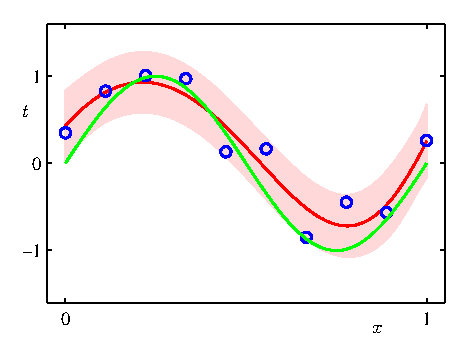
\includegraphics[width=8cm]{Figure1-17.eps}}
	\end{figure}
	
\section{模型选择}
	在我们使用最小二乘法来进行多项式曲线拟合的例子里面,我们可以看到当选择最优的多项式的阶时,会得到最好的生成结果。多项式的次数控制了模型的自由度,因而控制了模型的复杂度。使用归一化的最小二乘法,归一化系数$\lambda$也控制了模型的有效复杂度,然而对如分布和神经网络的混合模型来说,或许会由多个参数来控制复杂度。在实际的应用中,我们需要确定这些参数的值和主要的目标,就可以实现对于新数据的最好预测性能。更多的,对于给定模型的情况下,找到复杂性参数的近似值,,我们希望考虑模型的不同类型的范围来找到我们应用的最好模型。
	
	我们从前面已经发现,在最大似然方法中,训练数据集的性能对未知数据集的预测性能不能得到好的指示,因为具有过拟合的问题。如果数据很多,一种简单的方法是使用一部分的可用数据来训练一个模型的范围,或者是具有一定范围的复杂度参数值的模型,然后用独立的数据来进行对比,这些数据有时候称为\textbf{确认集}(\textit{validation set}),最后选择一个具有最好预测性能的模型。如果模型设计用有限的数据集进行很多次的迭代,就可能在确认数据集中出现过拟合情况,因此很必要再保留一个称为\textbf{测试集}(\textit{test set})的数据集来选择最后的评估模型。
	
	然而在很多的应用中,训练和测试的数据集是有限的,为了找到一个最好的模型,我们希望能最大限度地使用数据来进行训练。然而,如果确认集太小,会得到一个具有相对噪声估计的预测性能。这种困境的一个解决方法就是使用交叉集,在图1.18中进行描述。这允许使用可用数据的一个比例$(S - 1)/S$来进行训练,用所有的数据来进行性能评估。当缺乏数据时,可能会近似地考虑$S = N$,其中\textit{N}是所有数据的点数,这种方法称为\textbf{留一法}(\textit{leave-one-out})。
	
	交叉验证的一个主要缺点是训练运行的次数随着因子\textit{S}的增加而增加,这种方法是有问题的,训练的代价太高。使用独立的数据来评估性能的交叉验证方法也有这样另一个问题,就是对于一个简单的模型,我们可能会有很多复杂性参数(如我们可能有几个归一化参数)。在最坏情况下,这种设置的结合可能会导致训练次数达到参数数量的指数情况。我们需要一个更好的方法。理想情况是应该只依赖训练集,并且允许在单次训练运行下对多元超参数和模型类型进行比较。因此我们需要找到一个性能测量方法,使得这种方法只依赖于训练数据,不会因为防止过拟合的原因遭受偏差情况。
	
	历史上已经提出了各种信息标准,通过对更复杂的模型增加惩罚项来矫正最大似然的偏差。例如\textbf{赤池信息准则}(\textit{Akaike information criterion}),也称为AIC (Akaike, 1974)通过下面量的最大值选择模型
	
	\begin{equation}
	\ln p(\mathcal{D}| \textbf{w}_{ML}) - M
	\end{equation}
	
	这里的$p(\mathcal{D}| \textbf{w}_{ML})$是最佳适合的对数似然,M是模型中可调整参数的数量。这种量的一个变形,称为\textbf{贝叶斯信息准则}(\textit{Bayesian information criterion})或者\textit{\textbf{BIC}}会在4.4.1节进行讨论。这种方法不会考虑模型参数中的不确定性,而是趋向于一个简单的模型。在3.4节中我们会转向全贝叶斯方法,那时我们将会看到复杂的惩罚项如何自然而由原理地提出。
	
\section{维灾难}
	
	
	